% -*- encoding: UTF8 -*-
%%*****************************************************************************
%%									                    	Theoretical Basics								 
%%*****************************************************************************
%
%
\chapter{Theory}
\label{Ch:Theory}	

\section{Optics}

\subsection{Point Scanned Imaging}
General characteristics

Sampling (nyquist)

\subsubsection{Confocal}

Confocal equations and PSF

\begin{figure}[h!]\centering \includegraphics[width=10cm,draft]{figures/foo.png}
      \caption{Probe with in confocal imaging mode and PSF}
      %\label{}
\end{figure}


\subsubsection{OCT}
OCT Equations

\begin{figure}[h!]\centering \includegraphics[width=10cm,draft]{figures/foo.png}
      \caption{OCT Schematic}
      %\label{}
\end{figure}


\newpage
\section{Mechanics of fiber scanners}

\subsection{Resonant Beam Theory}
\label{sec:EB}
Following the Euler-Bernoulli theory \cite{MarcJ.Madou2011}, the spring constant for a fixed-free, point loaded cantilever is given by 
\begin{equation}
K_\mathrm{cantilever} = \frac{3 E I}{L^3} = \frac{3 \pi}{4} \frac{E_\mathrm{fiber} r_\mathrm{fiber}^4}{L^3}
\label{eq:EB}
\end{equation}
considering that the moment of inertia of the cylindrical fiber is given by $I_\mathrm{fiber} = \frac{\pi}{4} r^4$.



The fiber-GRIN assembly can be modeled as a point-loaded, fixed-free cantilever and the GRIN lens weight can be concentrated in its center of gravity, as depicted in Figure \ref{fig:EB}). 
\begin{figure}[h!]\centering
      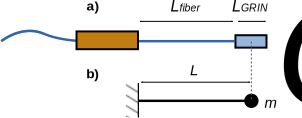
\includegraphics{figures/30_DesignSimulation/Mechanical/EB.pdf}
      \caption{\textbf{a)} Drawing of the piezoelectricscanner: piezoelectric tube, fiber and GRIN lens. 
      \textbf{b)} Simplified mechanical diagram obtained by modeling the fiber as a weightless cantilever and the GRIN lens as a point mass.}
      \label{fig:EB}
\end{figure}
Now, by applying the ideal mass-spring harmonic resonator equation 
\begin{equation}
f_\mathrm{res} = \frac{1}{2 \pi} \sqrt{\frac{K_\mathrm{cantilever}}{m_{\mathrm{GRIN}}}} 
\label{eq:fres}
\end{equation}

\begin{figure}[h!]
      \centering
      \includegraphics[width=10cm,draft]{figures/foo.png}
      \caption{CAD Drawing > Mechanical Modeling}
      %\label{}
\end{figure}
Euler-Bernoulli description of resonant beam

Theoretical resonance frequency 

Angular deflection


\subsection{Piezoelectric Tube Actuators}



\begin{figure}[h!]
      \centering
      \includegraphics[width=10cm,draft]{figures/foo.png}
      \caption{Side view: Bimorph actuator / Cross section of piezo tube with fields / Equivalent electric circuit}
      %\label{}
\end{figure}